% use paper, or submit
% use 11 pt (preferred), 12 pt, or 10 pt only

\documentclass[letterpaper, preprint, paper,11pt]{AAS}	% for preprint proceedings
%\documentclass[letterpaper, paper,11pt]{AAS}		% for final proceedings (20-page limit)
%\documentclass[letterpaper, paper,12pt]{AAS}		% for final proceedings (20-page limit)
%\documentclass[letterpaper, paper,10pt]{AAS}		% for final proceedings (20-page limit)
%\documentclass[letterpaper, submit]{AAS}			% to submit to JAS

\usepackage{bm}
\usepackage{amsmath}
\usepackage{subfigure}
%\usepackage[notref,notcite]{showkeys}  % use this to temporarily show labels
\usepackage[colorlinks=true, pdfstartview=FitV, linkcolor=black, citecolor= black, urlcolor= black]{hyperref}
\usepackage{overcite}
\usepackage{footnpag}			      	% make footnote symbols restart on each page
\usepackage{float}



\PaperNumber{XX-XXX}


\begin{document}

\title{\textsf{\textbf{Induced Fragmentation of Asteroids during Close Encounters}}}
\author{\textsf{Bryan Tester}\thanks{(bryan.tester@strath.ac.uk) PhD student at University of Strathclyde, United Kingdom}
\ and \textsf{Prof. Massimiliano Vasile}\thanks{(massimiliano.vasile@strath.ac.uk) Professor at University of Strathclyde, United Kingdom}}

\maketitle{} 		


\begin{abstract}
We consider the behaviour of rotating binary asteroids as they pass through Earth's Hill sphere, with primary interest in the effect the tidal force on the interaction between the two components of the binary and their post-encounter trajectories. We focus on contact binary asteroids bound by a regolith bridge, using both direct numerical simulation and analytical approaches to investigate the sensitivity of the system to different parameters. We find that the system is most sensitive to the angle between the binary pair and the orbital path, having a significant impact upon the energy change during a fragmentation event. We also give the results of some basic simulations of a deflection attempt on such an object.
\end{abstract}

\section{Introduction}
Radar observations suggest that a significant portion of asteroids with Earth-crossing orbits are binary systems, consisting of two components in contact with or in close proximity of each other. As shown by work such as that of Farinella \textit{et al} \cite{binaryevo} in the early 1990s, gravitational encounters can significantly alter the orbits and integrity of such binary systems. It is important to be able to accurately predict the motion of these bodies for maximum warning of any possible Earth collision event. The main effect we consider here is the "Binary Exchange" mechanism, as discussed by Borum \textit{et al}\cite{exchange}. This is where a rotation of a binary pair is disrupted by the tidal forces, causing the pair to split and altering the orbital energy of each component. 

In this work, we consider “Contact Binaries”; single asteroids formed primarily by two large boulders. We consider both gravitationally bound pairs and those bound by a "regolith bridge", as illustrated in Figure ~\ref{fig:Pic}. The bridge is comprised of many small dust particles; the size of which cause in non-negligble London Dispersion forces between them resulting in adhesive effect between them and the larger components (This mechanism is similar to that discussed by Sanchez \& Scheeres \cite{dustbound}). We also model an attempted deflection of the binary system to the close encounter, using and impactor-type method. This work forms a theoretical basis in the event such a deflection mission is required.

\begin{figure}[H]
\centering
\includegraphics[width=0.8\textwidth]{binary_3d.eps} 
\caption{Simulation of two large spheres joined by a finer regolith bridge.} 
\label{fig:Pic}
\end{figure} 

The analytical work starts with the full equations of motion for a binary system in a non-inertial reference frame rotating about the centre of the Earth. We use a standard virtual forces method, incorporating the Centrifugal, Coriolis and Euler forces to account for the rotation of the frame. Using a series of relevant approximations, the equations are simplified to give a handle on the factors that have a significant impact on the system. The numerical simulations are performed using a custom multi-body code that includes full inter-particle gravitational interactions, London dispersion forces and Soft-Body collisions similar to those implemented in \textit{PKDGRAV} by Schwartz \textit{et al}\cite{soft}. Previous work on the orbits of binary and rubble pile asteroid system are performed with modeling limited to only the gravitational interactions between the components. 

The first set of simulations include only the two binary components and Earth. Simulations are performed for a range of binary system rotation speeds and two-body energies. The first set places the binary components are in a mutual circular orbit with artificially varies force between them to simulate the effects of a regolith bridge or other forces binding the two components. The second set of simulations include a full regolith bridge \textbf{\emph{I think you should mention the physics you are using for simulating the forces that keep the regolith and binary components together}}.

\textbf{\emph{Max usually likes a paragraph here giving the structure of the paper}}.

\section{Equations of Motion}

\textbf{\emph{See above comment on reference frame}}. The analytical approach to characterising the system is based upon the full equations of motion in a rotating reference frame, with the angular velocity of the reference frame $\vec{\omega}$ varying such that the barycentre of the system remains at a constant angle to the Earth. We define the binary in terms of the position of its barycentre $\vec{R}$, and the vector $\vec{\rho}$ such that the two components are located at $\vec{R}\pm\vec{\rho}$ (the two components are considered to be identical, both of mass $m$ and radius $r$). Using the standard non-inertial forces for a rotating frame (Centrifugal, Coriolis and Euler), we obtain the following equation:
\begin{equation}
\ddot{\vec{R}}\pm\ddot{\vec{\rho}} = -\frac{GM_\oplus(\vec{R}\pm\vec{\rho})}{\|\vec{R}\pm\vec{\rho}\|^{3}} + \left[\frac{-Gm}{4\|\vec{\rho}\|^{3}}+F(\vec{\rho})\right]\vec{\rho} +  \vec{\omega}\times[2(\dot{\vec{R}}\pm\dot{\vec{\rho}}) + \vec{\omega}\times(\vec{R}\pm\vec{\rho})]+\dot{\vec{\omega}}\times(\vec{R}\pm\vec{\rho}) 
\end{equation}
The resulting equation can be split into two separate parts, detailing the motion of the barycentre and the relative motion of the binary components respectively ($\vec{\rho_{\pm}}$ denotes the acceleration relative to the barycentre of the binary component located at $\vec{R}\pm\vec{\rho}$).
 
\begin{equation}
\ddot{\vec{R}} = \frac{-GM_\oplus}{\|\vec{R}\|^{3}}\vec{R}+\vec{\omega}\times(2\dot{\vec{R}}+\vec{\omega}\times\vec{R})+\dot{\vec{\omega}}\times\vec{R}
\end{equation}

\begin{equation}
\ddot{\vec{\rho}}_{\pm} = \left[\frac{-Gm}{4\|\vec{\rho}\|^{3}}+F(\vec{\rho})\right]\vec{\rho}+\vec{\omega}\times(2\dot{\vec{\rho}}+\vec{\omega}\times\vec{\rho})+\dot{\vec{\omega}}\times\vec{\rho}+{GM_\oplus}\left[\frac{\mp\vec{R}}{\|\vec{R}\|^{3}}-\frac{\vec{R}\pm\vec{\rho}}{\|\vec{R}\pm\vec{\rho}\|^{3}}\right]
\end{equation}

We start our analysis by working with the equation of motion for $\vec{R}$; as stated earlier, the definition of $\vec{\omega}$ in our reference frame implies that the direction of $\vec{R}$ is constant. Thus, any components of $\vec{\ddot{R}}$ orthogonal to $\vec{R}$ must be zero. This implies the following definiton of the magnitude of $\vec{\ddot{R}}$, along with equation 3 (which is equivalent to the conservation of angular momentum): 
\begin{equation}
\ddot{R} = \frac{-GM_\oplus}{R^{2}}+\omega^{2}R
\end{equation}
\begin{equation}
2\vec{\omega}\times\dot{\vec{R}}+\dot{\vec{\omega}}\times\vec{R}=0
\end{equation}
Since we consider no forces acting outside of the orbital plane, the direction of $\vec{\omega}$ must remain constant and orthogonal to $\vec{R}$ at all times. We consider the conservation of angular momentum to obtain an equation for $\omega$ (the magnitude of $\vec{\omega}$):
\begin{equation}
\frac{\partial\left(R^{2}\omega\right)}{\partial t} = 2R\dot{R}\omega + R^{2}\dot{\omega} = 0 \implies R^{2}\omega = constant
\end{equation}
Assuming the initial values $R_0$ and $\omega_0$ at some time $t_0$ we get the following:
\begin{equation}
\omega = \frac{R_0^{2}\omega_0}{R^{2}}
\end{equation}

Now, we consider the equation of motion for the position of the binary components relative to the centre of mass, $\vec{\rho}$. We chose to work solely with the equation describing the motion of the component located at $\vec{R}+\vec{\rho}$; an analysis could be performed for the other component but similar results would be expected. We make the assumption that the pair remains in a mutual circular orbit until the fragmentation event occurs. As such, by considering only components of the vector acting in the $\vec{\rho}$ direction we obtain an equation describing the forces responsible for the binding of the pair ($\theta$ being the angle between $\vec{R}$ \& $\vec{\rho}$ at a given time).
\begin{equation}\label{eq:rdd}
\ddot{\rho} = \left[\frac{-Gm}{4\rho^{2}}+F(\rho)\right]+2\omega\dot{\rho}+\omega^{2}\rho+{GM_\oplus}\left[\frac{\cos\theta}{R^{2}}-\frac{R\cos\theta+\rho}{(R^{2}+2R\rho\cos\theta+\rho^{2})^\frac{3}{2}}\right]
\end{equation}

If we consider the fragmentation event to be instantaneous and that the radius of the binary orbit remains constant up until this point, we can neglect the term involving $\dot{\rho}$ in equation~\ref{eq:rdd}. The resulting equation has two important parts; namely the attractive and repulsive terms.
\begin{equation} \label{eq:attr}
\ddot{\rho}_{attr} = \left[\frac{-Gm}{4\rho^{2}}+F(\rho)\right]
\end{equation}
\begin{equation} \label{eq:rep}
\ddot{\rho}_{rep} = \omega^{2}\rho+{GM_\oplus}\left[\frac{\cos\theta}{R^{2}}-\frac{R\cos\theta+\rho}{(R^{2}+2R\rho\cos\theta+\rho^{2})^\frac{3}{2}}\right]
\end{equation}
The attractive force remains constant throughout the orbit, whereas the repulsive force varies with distance to the Earth, relative angle of the pair and orbital angular velocity. The sensitivity of the force to these parameters is investigated with full numerical simulations of such encounters. 


\section{Numerical Simulations}
\subsection{Multi-Body Code}
As mentioned previously, the numerical simulations are performed using a simple multi-body code that implements soft-body collisions and makes use of a Second-order "Leapfrog" simplistic integration scheme, much like the work of Schwartz \textit{et al}\cite{soft}. The code makes use of OpenCL to allow for the utilisation of multiple processor cores and the possibility of running the code on a GPU. 

The simulations incorporate gravitational interactions between all particles, as well as London dispersion forces. For point particles, the attractive and repulsive potentials that characterize the London dispersion interaction are proportional to ${1}/{r^6}$ and ${1}/{r^{12}}$, respectively. However, the formulation is more complicated for finite sized particles. Hamaker\cite{hamaker} gives a derivation of the attractive potential between two spheres, calculated as the integral of the forces between infinitesimal point-particle elements over both spheres. In principle, this integral could be applied also to the repulsive term. However, since we use a soft-body collision method, including this term would provide no additional accuracy. Instead, we use a Pseudo-potential method (detailed in Equation 9): for distances greater than a given cut-off radius $r_{cutoff}$, the full value of the Hamaker\cite{hamaker} potential is used; for distances less than $r_{cutoff}$, a quadratic function is used. The quadratic used is set to have the same value and gradient as the Hamaker\cite{hamaker} potential at the cut-off point, and a global minimum at some point $r_{min}$ that is set to be less than the sum of the radii of the two spheres, thus allowing some overlap and "softening" the potential. 
\begin{equation}
V(r) = \left\{
\begin{array}{lr}
-\frac{A}{6}\left(\frac{2R_iR_j}{r^2-[R_i+R_j]^2}+\frac{2R_iR_j}{r^2-[R_i-R_j]^2}+\log\frac{r^2-[R_i+R_j]^2}{r^2-[R_i-R_j]^2}\right) & : r > r_{cutoff}\\
\frac{V'_{cutoff}}{2(r_{cutoff}-r_{min})}(r-r_{min})^2+V_{cutoff} - \frac{V'_{cutoff}(r_{cutoff}-r_{min})}{2} & : r \leq r_{cutoff}
\end{array}
\right.
\end{equation}

\subsection{Simulation Results}

Using the code described, a series of simulations are performed to explore the dynamics of close encounters of binary asteroids with Earth-sized bodies. Before discussing specific results, we outline the setup considered and the nature of the output of the code.

The majority of our simulations consider a parabolic encounter with a closest approach distance of 130km. The simulation outputs a track of positions, velocities, kinetic and potential energies for each body considered. The data we primarily consider is the sum of kinetic and potential energies for each component individually;  Figure~\ref{fig:Num} shows a plot of this total energy for the two binary components produced by a simulation. After the fragmentation one components is "captured" (having its orbital energy reduced below zero) and the other escapes (gaining orbital energy). The break-up is observed as the energy trace transitions from the oscillating regime to a steady state; we define the fragmentation energy as the difference between the average total energy of a binary component and the final energy state. \textbf{\emph{OK, a lot of points to be considered here. Firstly, the font is too small in the figure. Also make the lines thicker.(Do this for all figure, line weight:3, font size 24). Also make sure all plots have legends. Mark on the figure the fragmentation event. Second, define simulation conditions, like velocity, size or something. Not sure what goes into the simulation, but you need to describe perhaps the orbital parameters. Basically, you need to provide anything someone would need in order to replicate the results. Plus, you are only showing results from one simulation, but in the text you mention as if you are performing multiple. If multiple, describe the conditions for each, if just one, you need to mention you are doing one simulation.}}
\begin{figure}[H]
\centering
\centerline{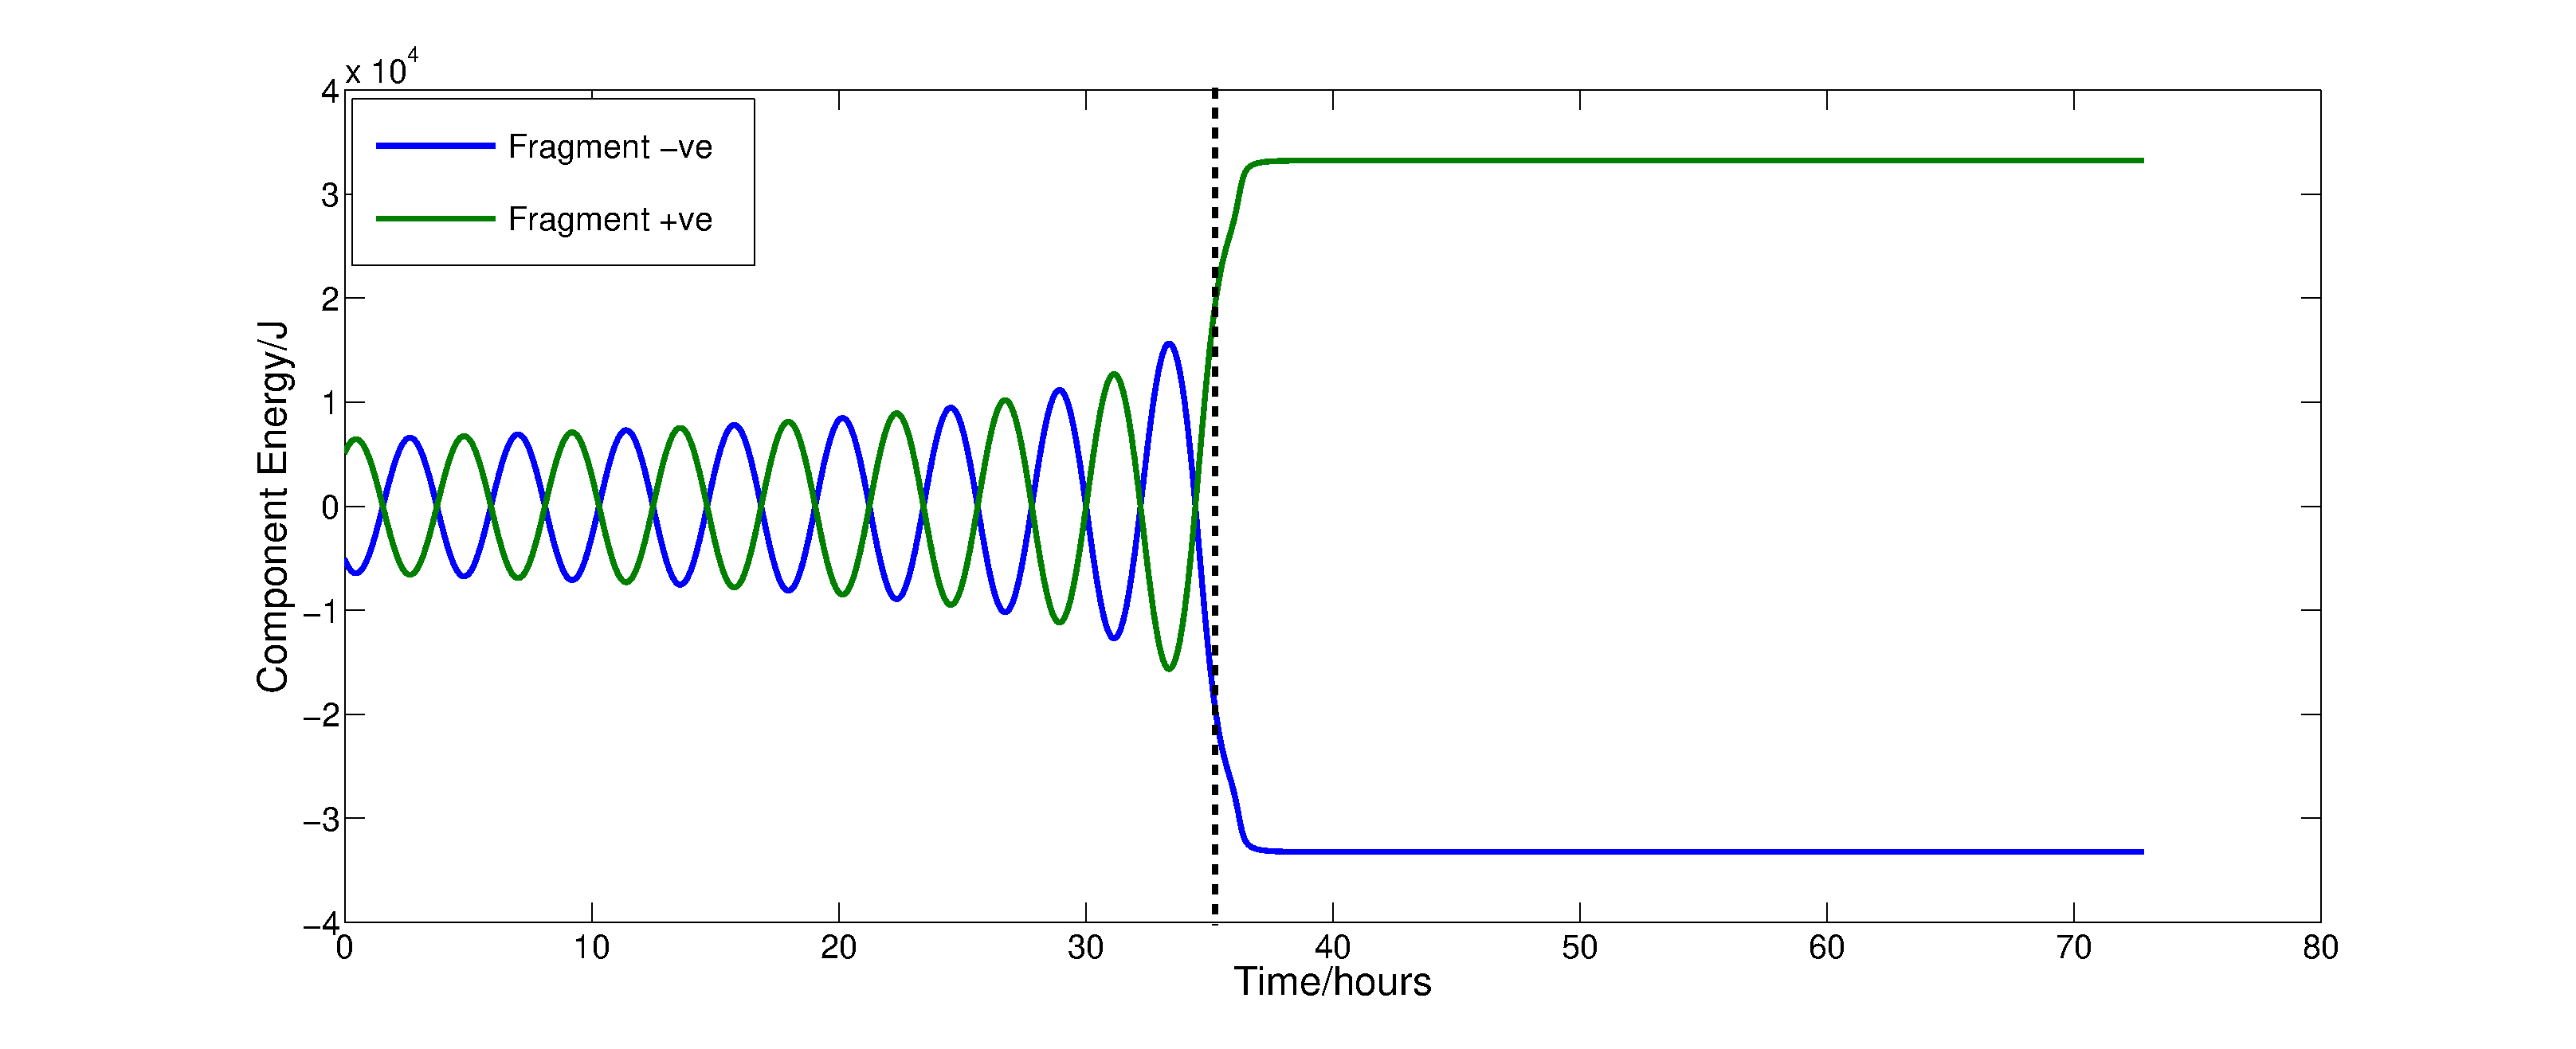
\includegraphics[width=1.2\textwidth]{binary_num.eps}} 
\caption{Plots of the Gravitational potential and kinetic energy of both components of the binary from numerical simulations.} 
\label{fig:Num}
\end{figure}
 

\subsection{Analytical Comparisons}

Using the set of equations derived earlier, we can make estimates for the behavior of the binary system. By running a series of simulations with varied initial conditions, we gauge the relationship between the fragmentation energy and the parameters $\theta$, $\omega$ \& $R$. Firstly, however, we attempt to verify the accuracy of some of the assumptions applied in the derivation of the equations; namely the constant rotation rate and radius of the binary pair prior to the fragmentation event. To do this, we run a simulation . \textbf{\emph{again, provide the simulation parameters. You need to do these for all simulations. Be consistent with legends and properties between the figure. Figure 3, provide label for Y axis, perhaps something like $\frac{X}{X_0}$. Again, mark the fragmentation event on the plot and provide a blowup as a PIP for the time before fragmentation since the scale does not show anything before fragmentation. When you say radius of a binary pair, are you talking about the distance of the barycenter, because technically after fragmentation, there should be two lines for both radius and angular speed}}.Figure~\ref{fig:omega} shows the radius and angular velocity of the binary pair over the course of an orbit. Prior to the fragmentation event, the fluctuation in angular speed is approximately 1\% of its magnitude.

\begin{center}
\begin{figure}[H]
\centering
\centerline{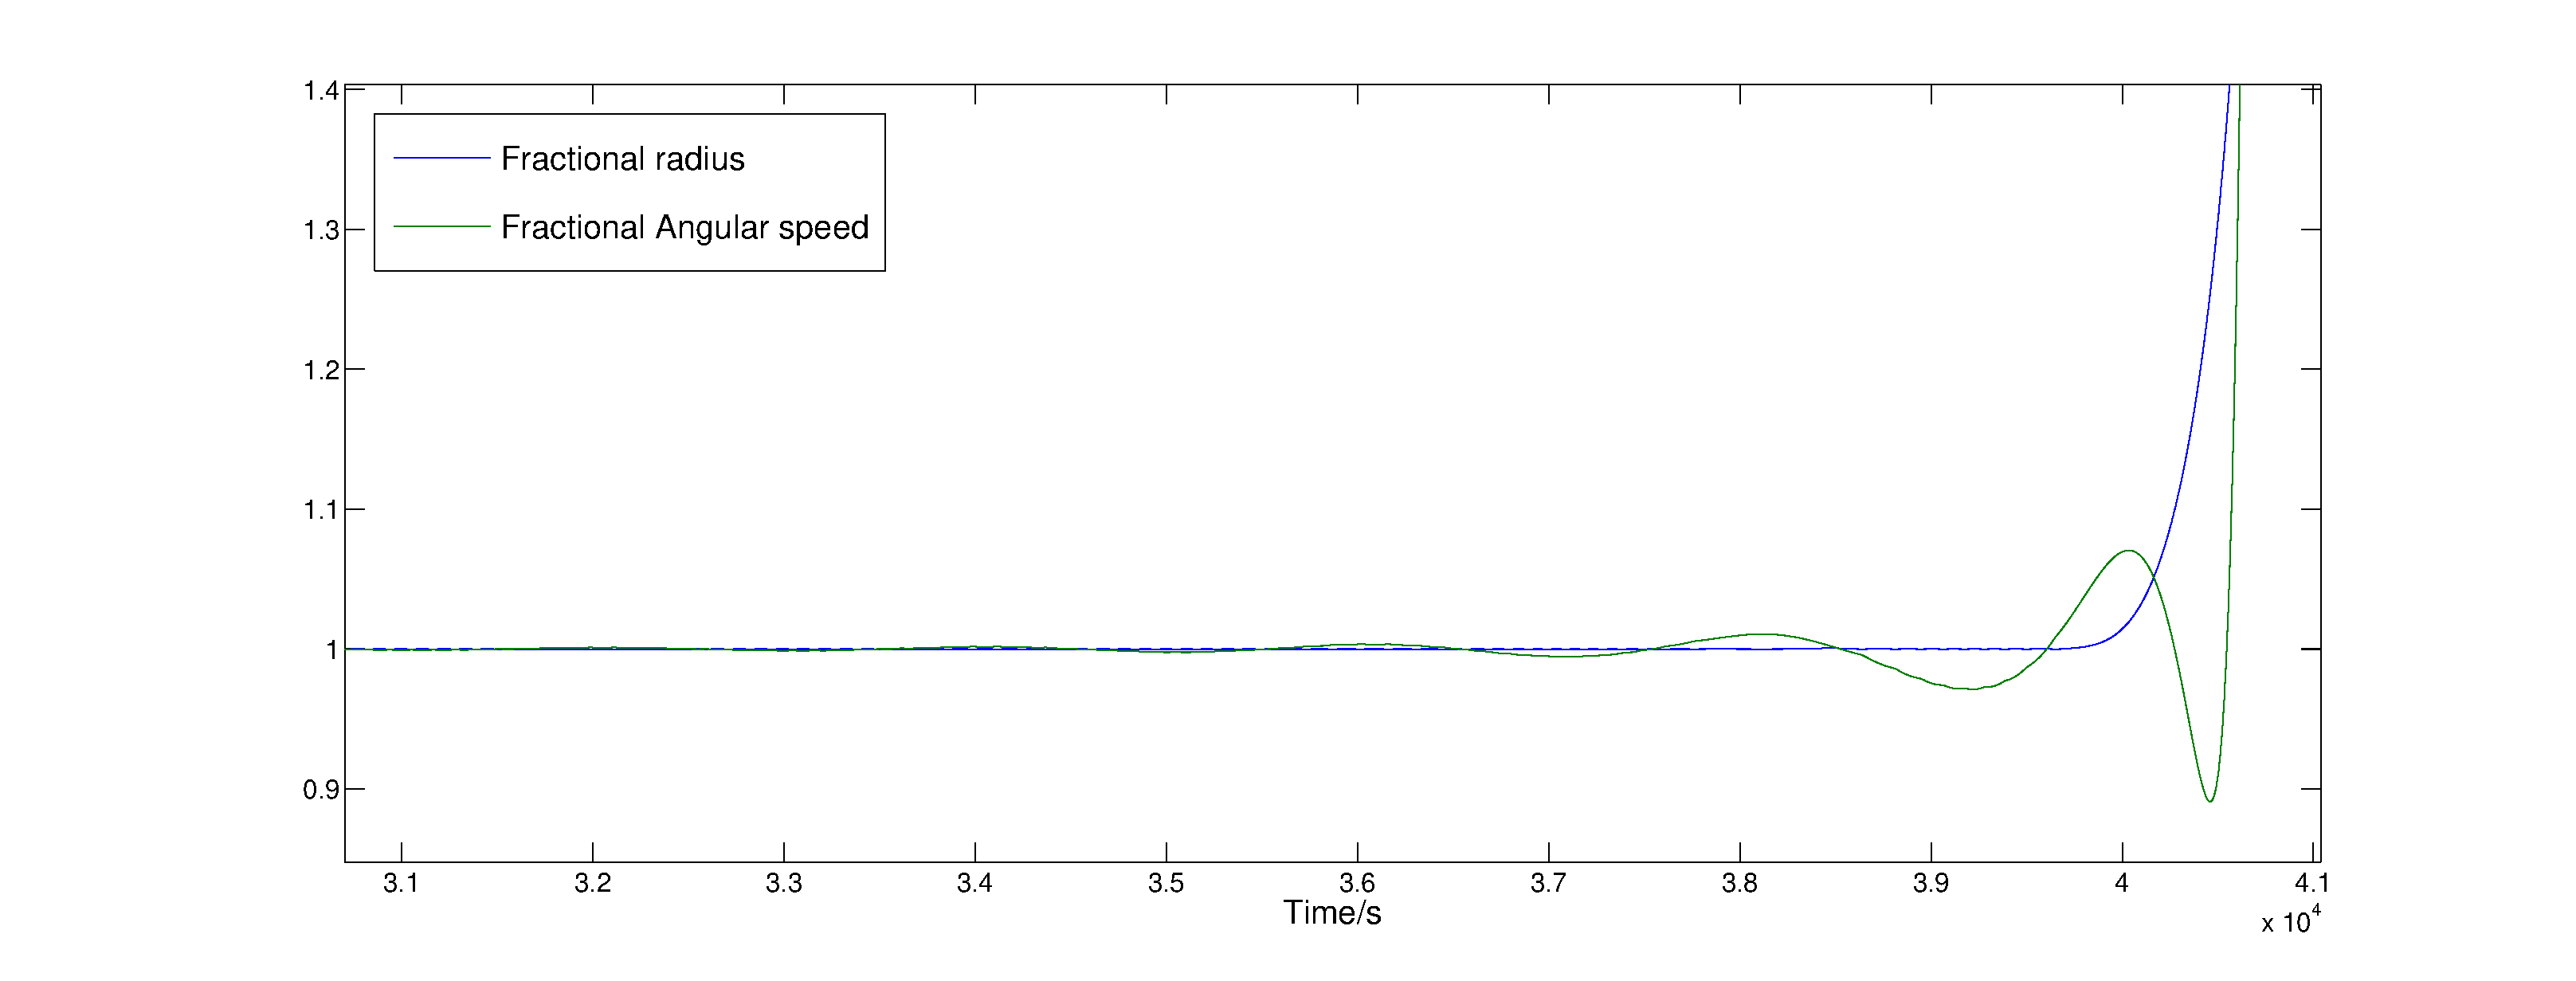
\includegraphics[width=1.2\textwidth]{omega.eps}} 
\caption{Plots of angular velocity and radius of a binary pair as fractions of the initial values.} 
\label{fig:omega}
\end{figure}
\end{center}

Now, we consider the sensitivity of the fragmentation energy to the parameters $\theta$, $\omega$ \& $R$. $\theta$ is varied by changing the starting orientation of the binary pair, whilst $\omega$ \& $R$ are changed by altering the orbital parameters. \textbf{\emph{Again, mention what conditions the last simulations were performed with and how you are changing those parameters (one at a time?), what range are you using for the parameters and why?}} Assuming the rotation rate is balanced with the attractive force between the binary components such that the orbit is circular when in free space (as is the case in all simulations presented here), any effective repulsive force between the two components introduced by the influence of a third body would alter the orbit into an elliptical one or if strong enough eliminate the possibility of any stable orbit. If the strength of the repulsive force is greater than that of the attractive, the net effective force between the pair is repulsive and as such fragmentation is inevitable. Figure ~\ref{fig:phase} shows the total energy plots for one component in a binary system over the course of an encounter with the Earth, with the value of $\theta$ at the start of the simulation varied. As can be seen, there is a significant variation in the final energy \textbf{\emph{with some cases getting captured while others escaping?}}. The discontinuities present in some curves are due to collisions between the components which occur as their orbit is destabilized. The relative velocity of these collisions is of the order of $10^{-4}m\cdot s^{-1}$,  so no destruction or deformation on the boulders is expected. As the angle varies steadily, the fragmentation energy initially varies as a small offset. However, as the value of $\theta$ at closest approach nears $\frac{\pi}{2}$ \textbf{\emph{how do we tell this from the figure?}}the energy varies more rapidly as the components "swap" (the one which gained orbital energy during the encounter for lower values of $\theta$ instead loses energy and vice versa).\textbf{\emph{can we explain why?}}
 \begin{figure}[H]
\centering
\centerline{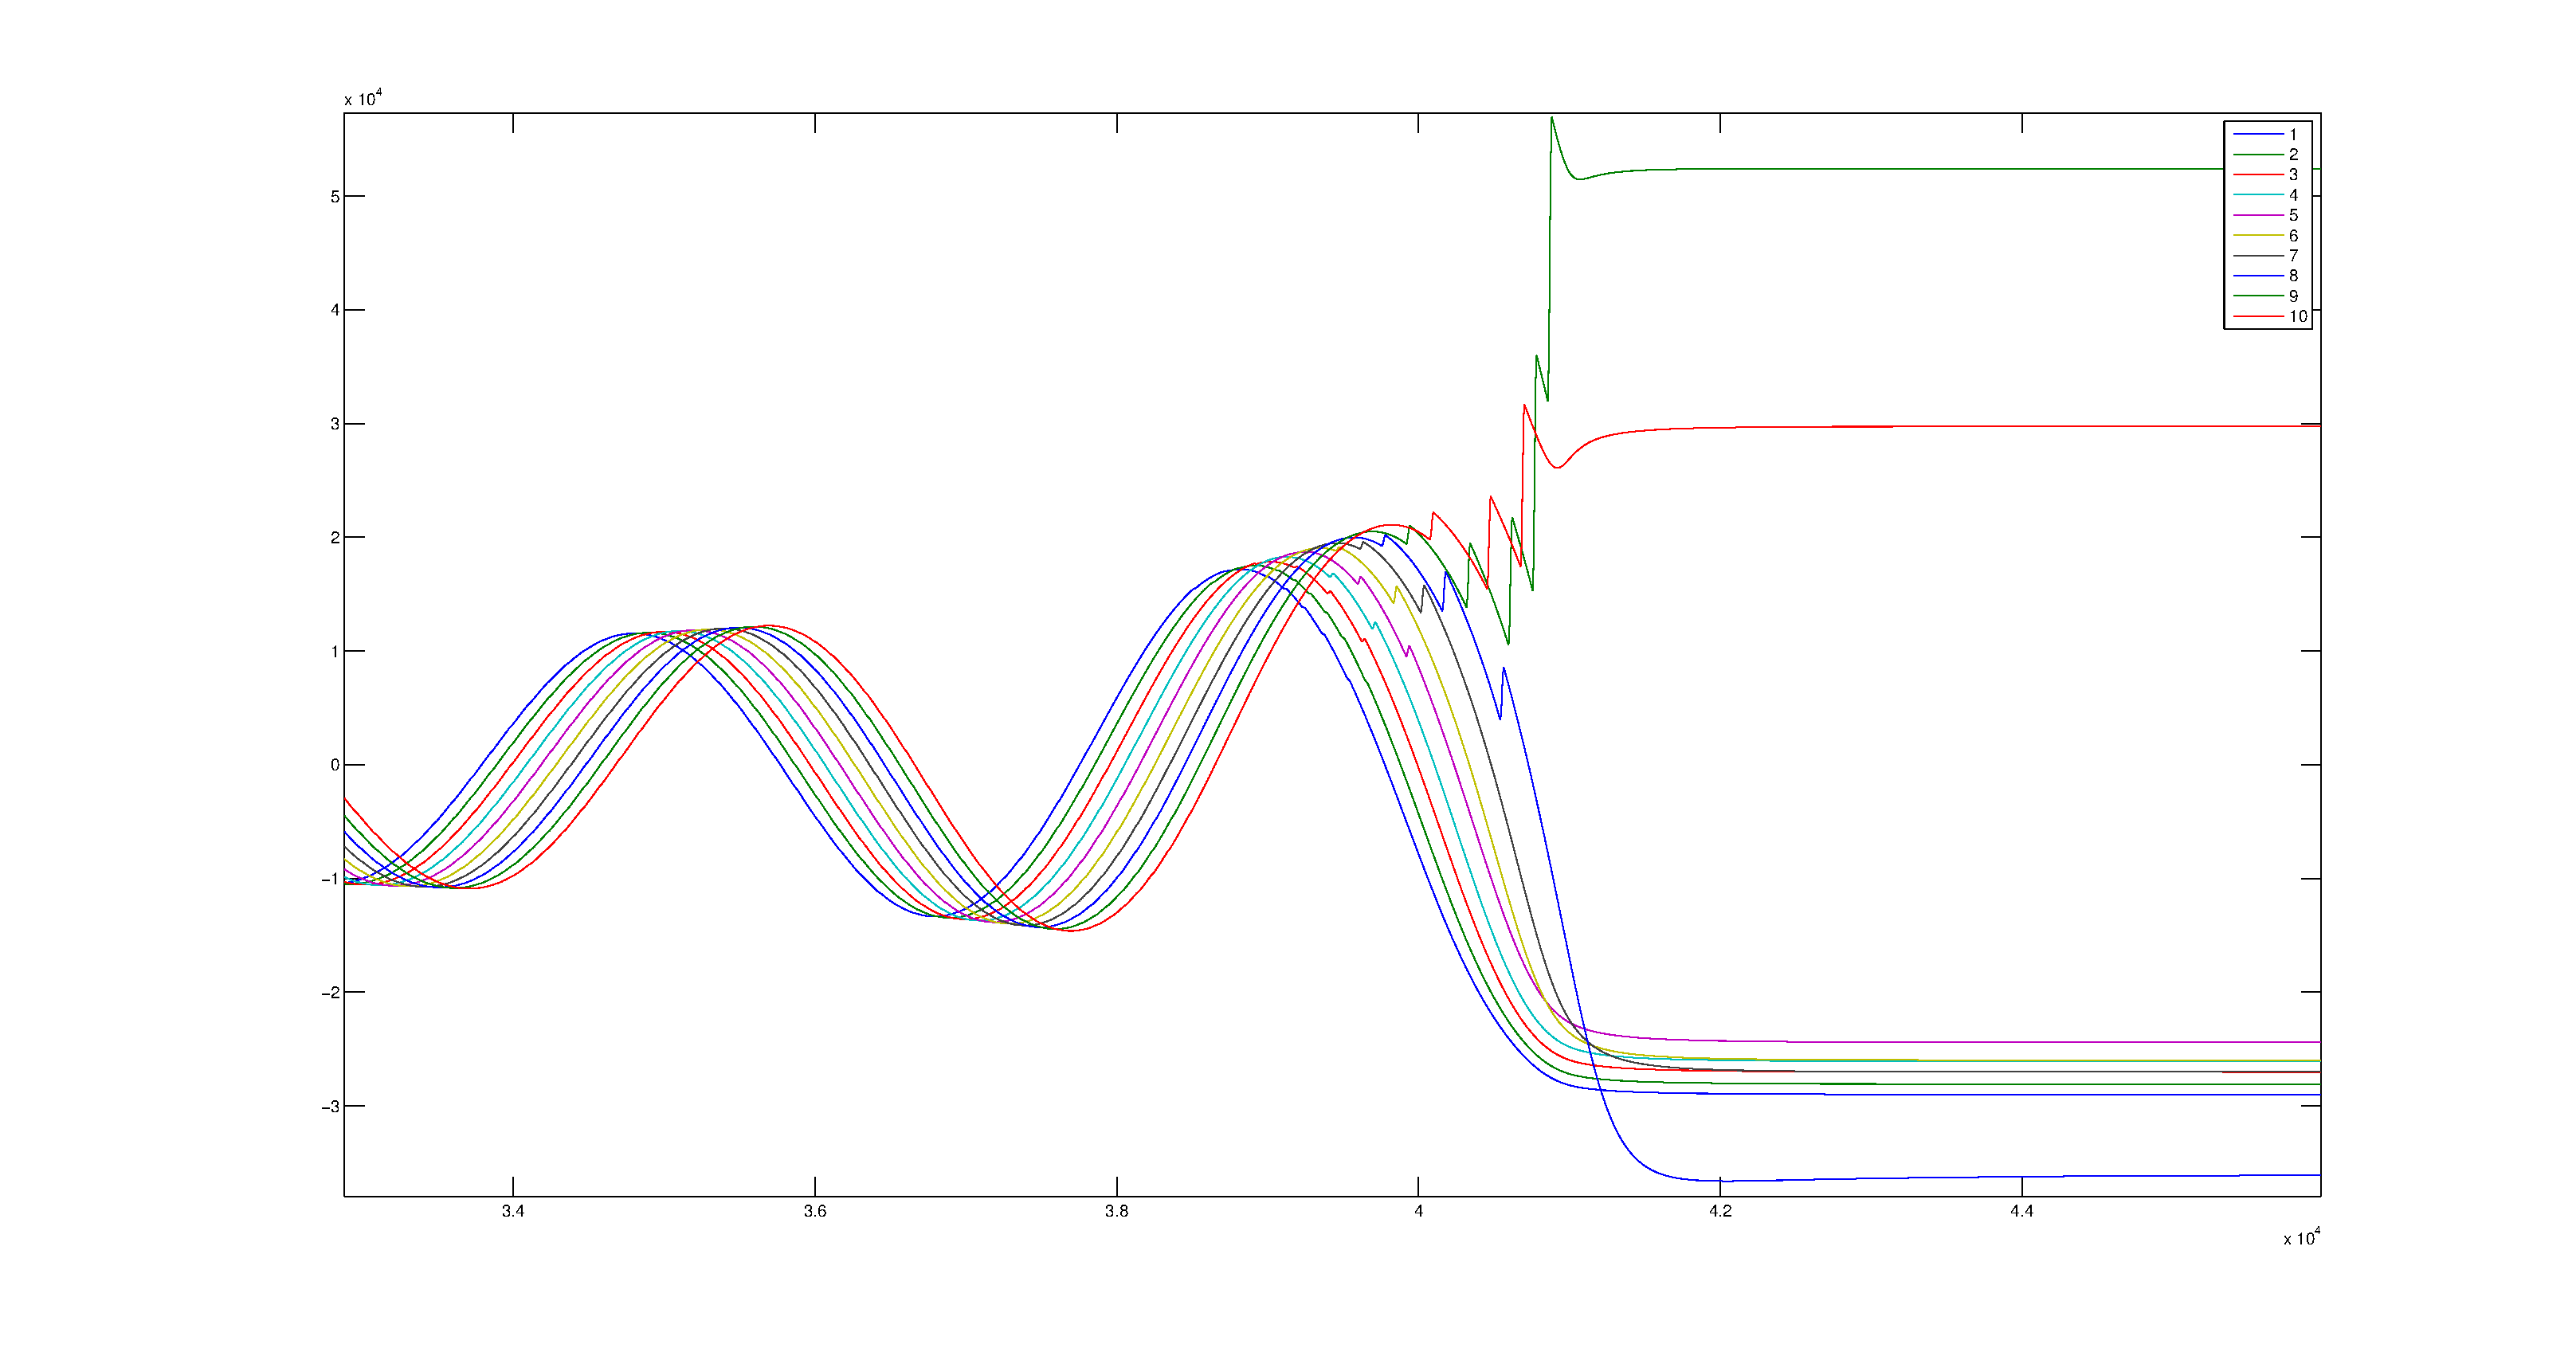
\includegraphics[width=1.2\textwidth]{phasing_2.eps}} 
\caption{Plots of the total energy for varying starting angle $\theta$.} 
\label{fig:phase}
\end{figure} 

For the analyses of both the $\omega$ and $R$ sensitivity, the setup is somewhat more complicated in principle as it is not possible to scale one without altering the other throughout the rest of the orbit. However, since the effects of the disruption will be greatest at the closest approach point, we change each parameter in uniform steps whilst keeping the other constant at this point. 
Using this procedure, the sensitivity of the fragmentation energy to the orbital speed $\omega$ is investigated. We maintain a constant closest approach distance of 130km but increase the orbital energy (and hence both the tangential and angular orbital velocity at this point). Figure~\ref{fig:omegasens} shows a plot of the energy traces of a single component for a range of values of $\omega$. As can be seen the fragmentation energy increases steadily with $\omega$ as would be expected from equation~\ref{eq:rep}. \textbf{\emph{Perhaps use more practical units in the figures, convert radians to degrees, seconds to minutes and meters to km}}
\begin{figure}[H]
\centering
\centerline{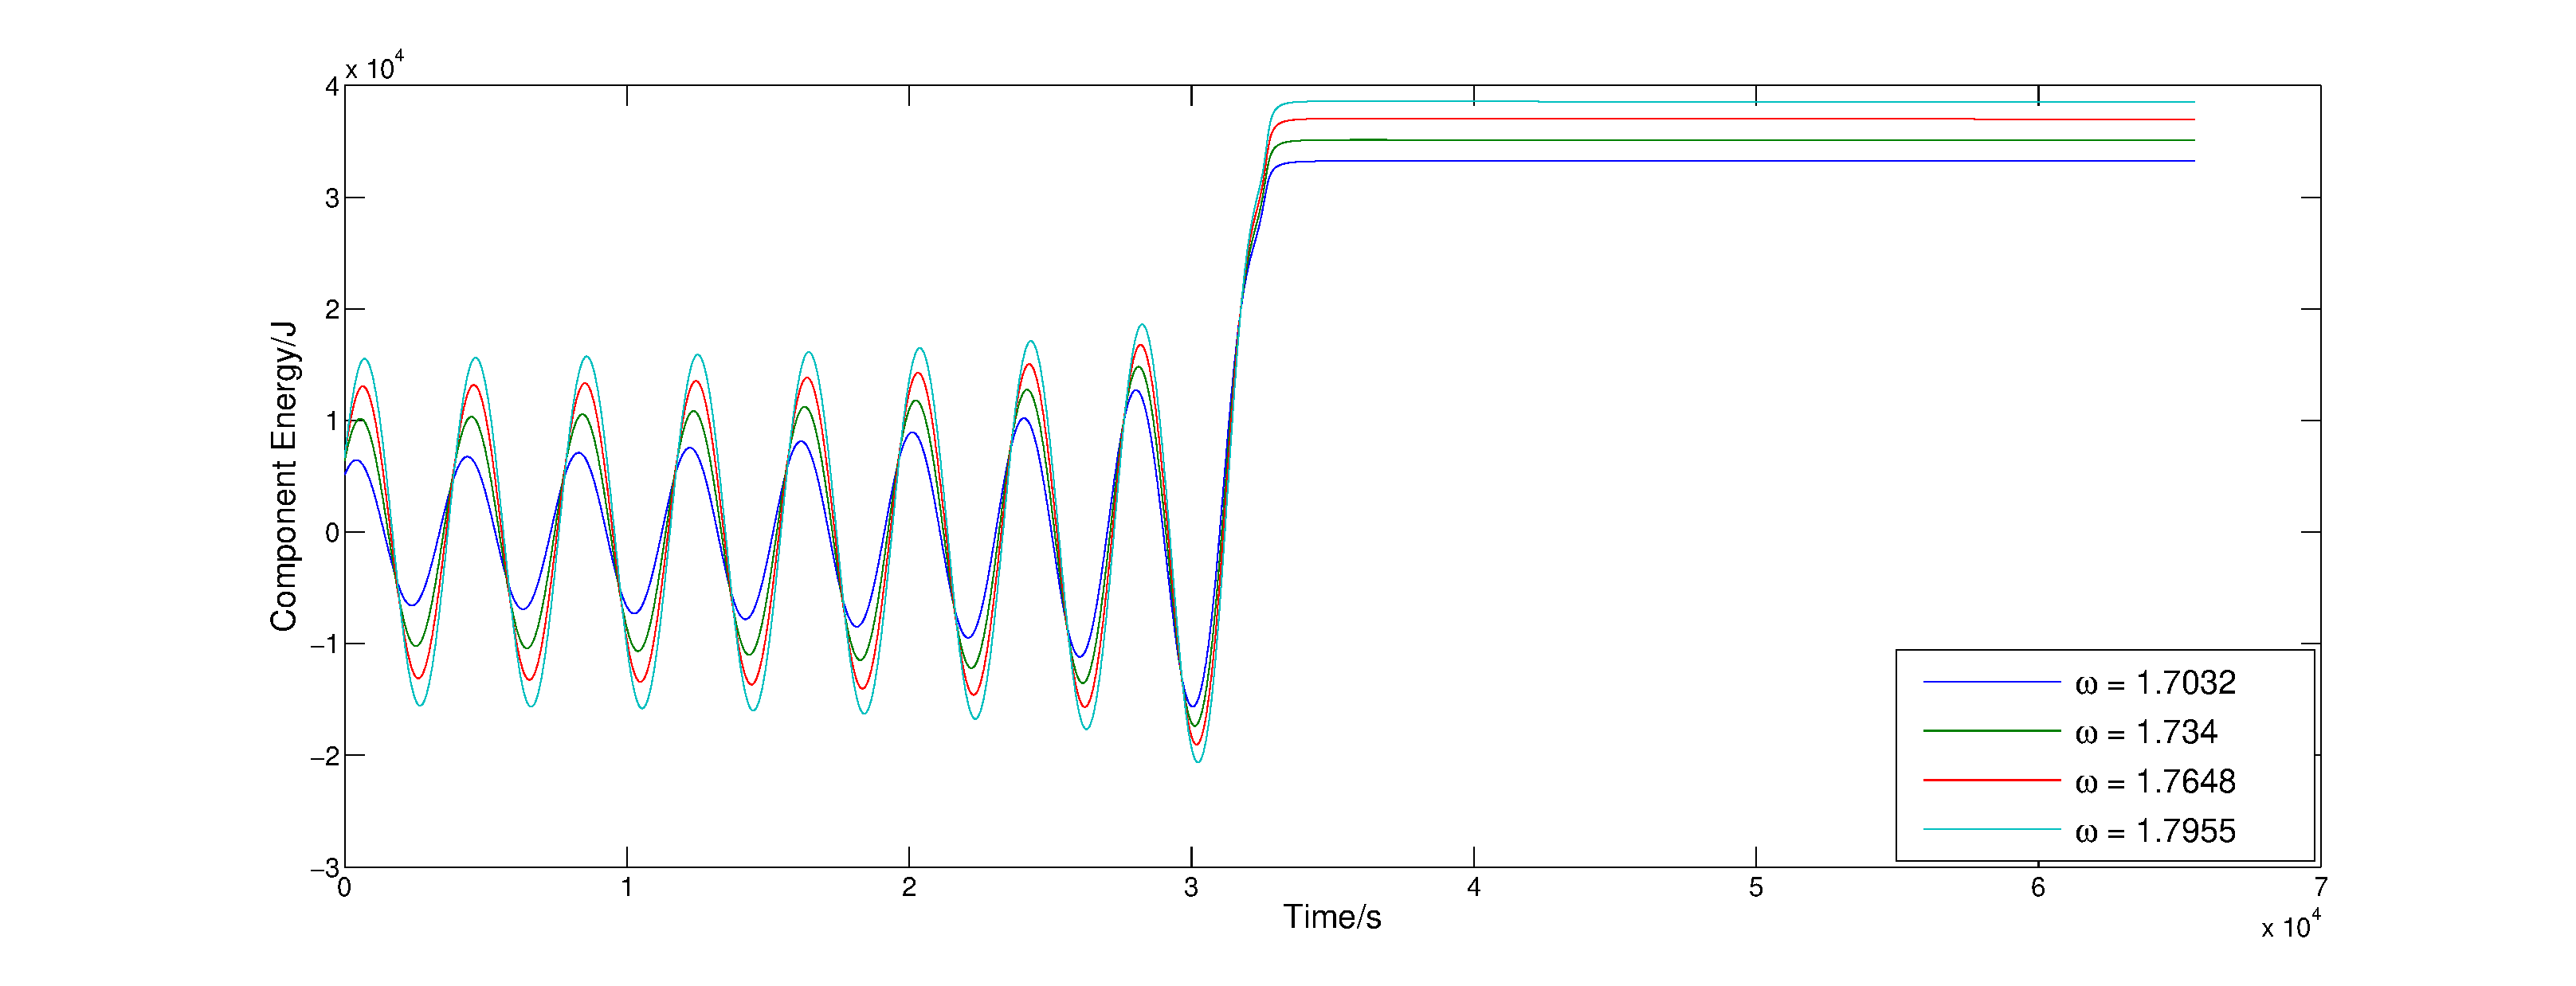
\includegraphics[width=1.2\textwidth]{omegasens.eps}} 
\caption{Plots of the total energy for varying orbital angular speed $\omega$ (values of $\omega$ in $mrad\cdot s^{-1}$).} 
\label{fig:omegasens}
\end{figure} 


Finally, we consider the sensitivity of the fragmentation energy to the Earth-Binary distance $R$. This is done by varying the closest approach distance whilst keeping the ratio between $R$ and $v$ at closest approach (and hence $\omega$) constant. As can be seen in figure~\ref{fig:Rsens}, the scaling of the fragmentation energy is smooth and increases with R;
\begin{figure}[H]
\centering
\centerline{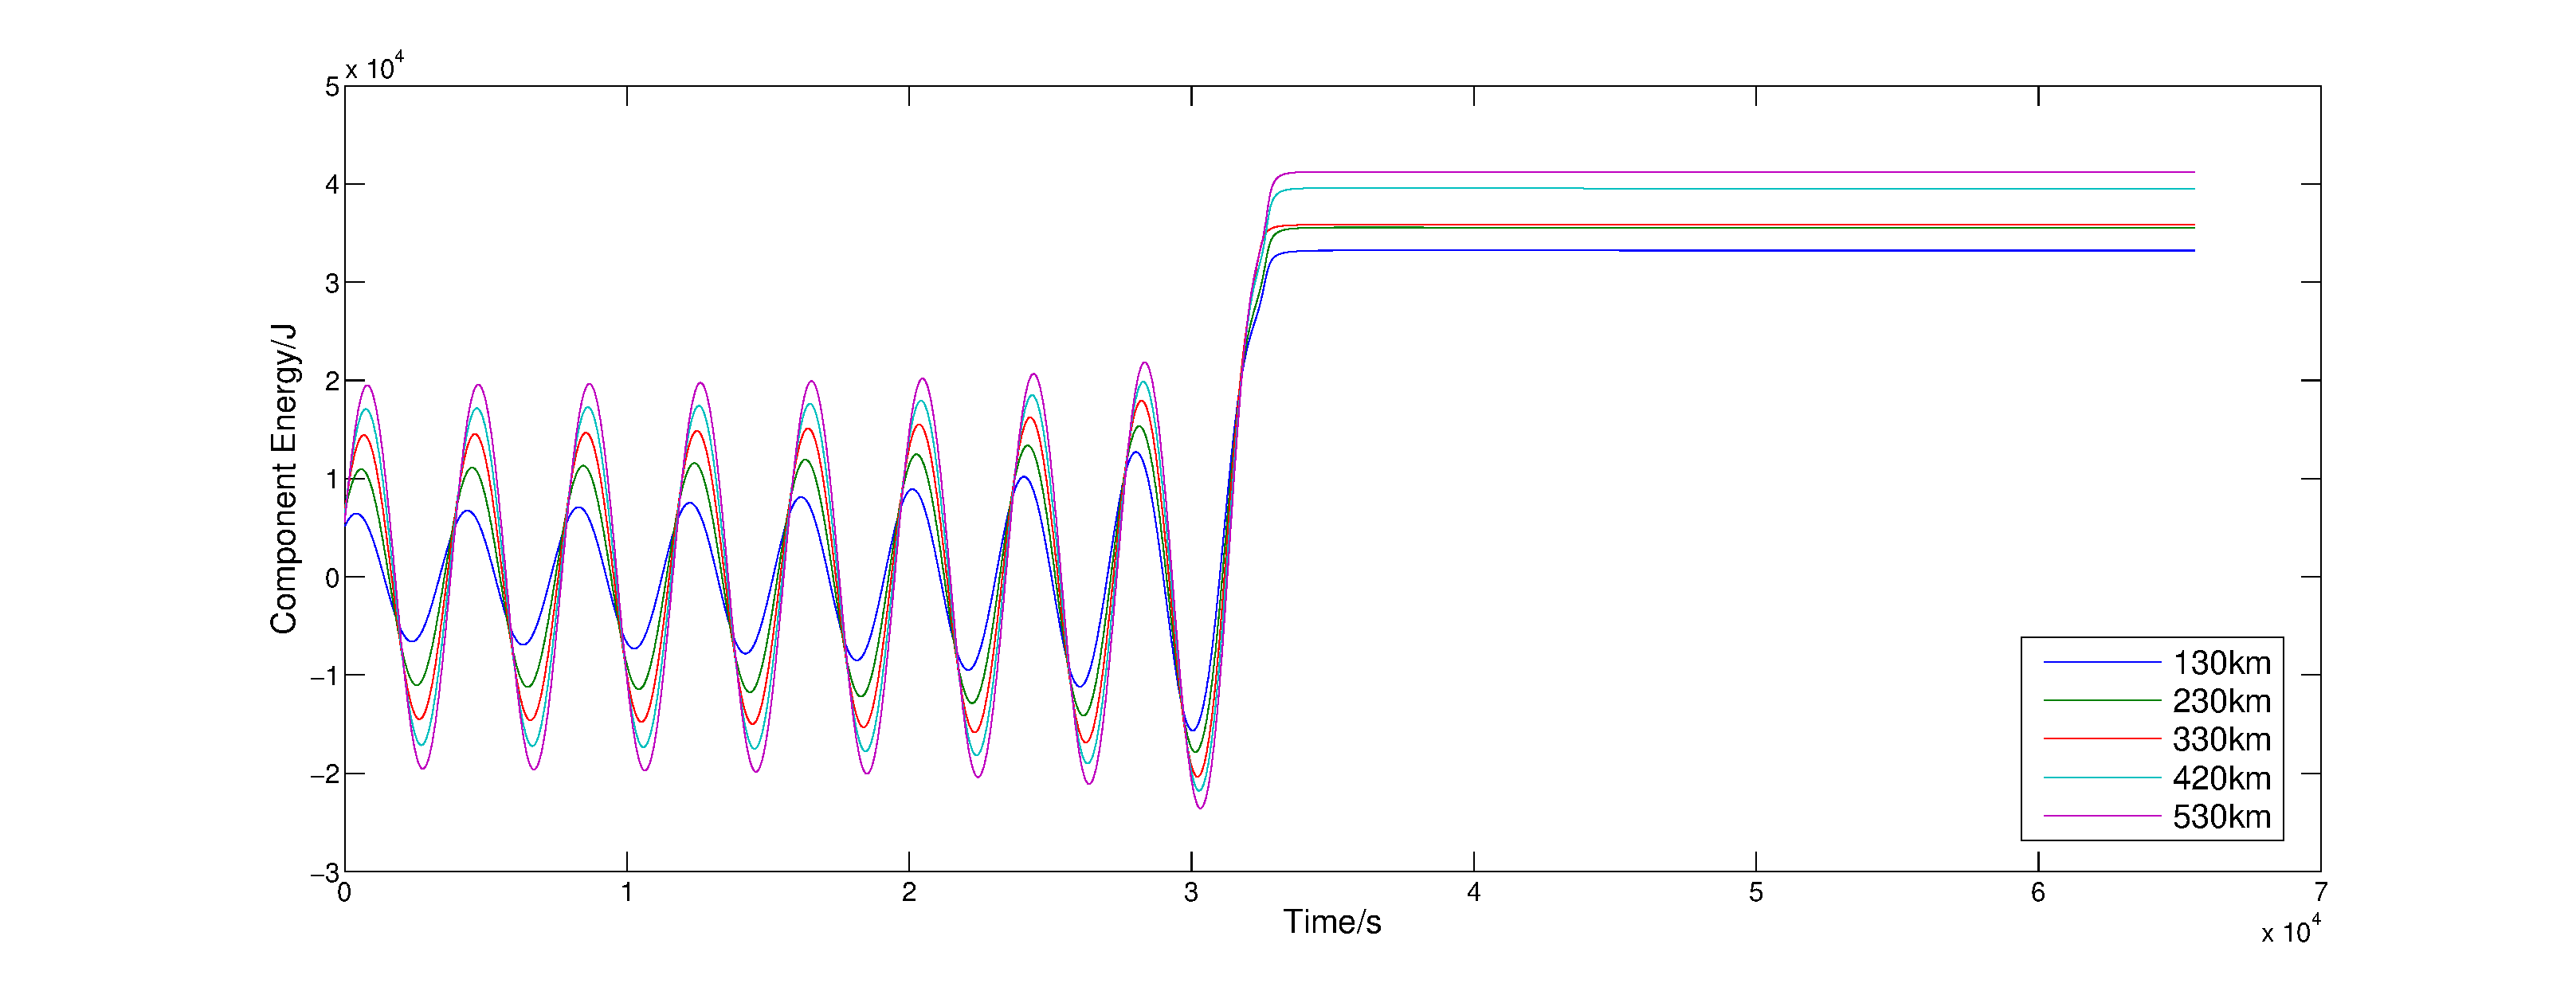
\includegraphics[width=1.2\textwidth]{Rsens.eps}} 
\caption{Plots of the total energy for varying closest approach distance $R$.} 
\label{fig:Rsens}
\end{figure} 


\subsection{Regolith-Bound Binary}
Following the sensitivity analysis \textbf{\emph{you never mention anywhere that you are doing a sensitivity study, probably a good idea to go back and describe it}}, numerical simulations of two boulders bound by a regolith bridge on a Parabolic trajectory are performed. For the small grain sizes considered in our regolith ($100\mu m$), the dominating force between particles are London Dispersion forces. Ideally, we wish to consider binary components with radii over 1 metre bound by a regolith bridge consisting of small ($100\mu m$) and medium ($1cm$) particles. However, the number of small particles that would need to be considered would make simulation of such a system not feasible. To overcome this, we first consider the binding effect between the small and medium particles. We perform a simulation with two medium sized granules bound by a bridge of 510 small particles. The system is placed under rotation, initially with the rotation speed matching that of a purely gravitational circular orbit for the two medium granules. The rotation rate is gradually stepped up until the binding of the granules fails. The value of the Hamaker\cite{hamaker} constant used in the simulation is then increased such that two medium sized granules have the same maximum rotation speed without the bridge as when bound by the small particulate bridge with the real value of the Hamaker\cite{hamaker} constant. A factor of approximately 200 was found to be sufficient; this is roughly equal to the number of small particles in contact with each medium granule. Figure~\ref{fig:dustyspin} shows the kinetic energy trace for a few key cases: rotation just below and just above the failure point of the bridge, and the same 2 rotation speeds but with the force approximation in place of the bridge. Hence, the system considered for the regolith-bound simulations is comprised of the larger binary components bound by a bridge of 510 medium sized granules, with the additional effect of the small particles approximated by increased strength of the London Dispersion force.  
\begin{figure}[H]
\centering
\centerline{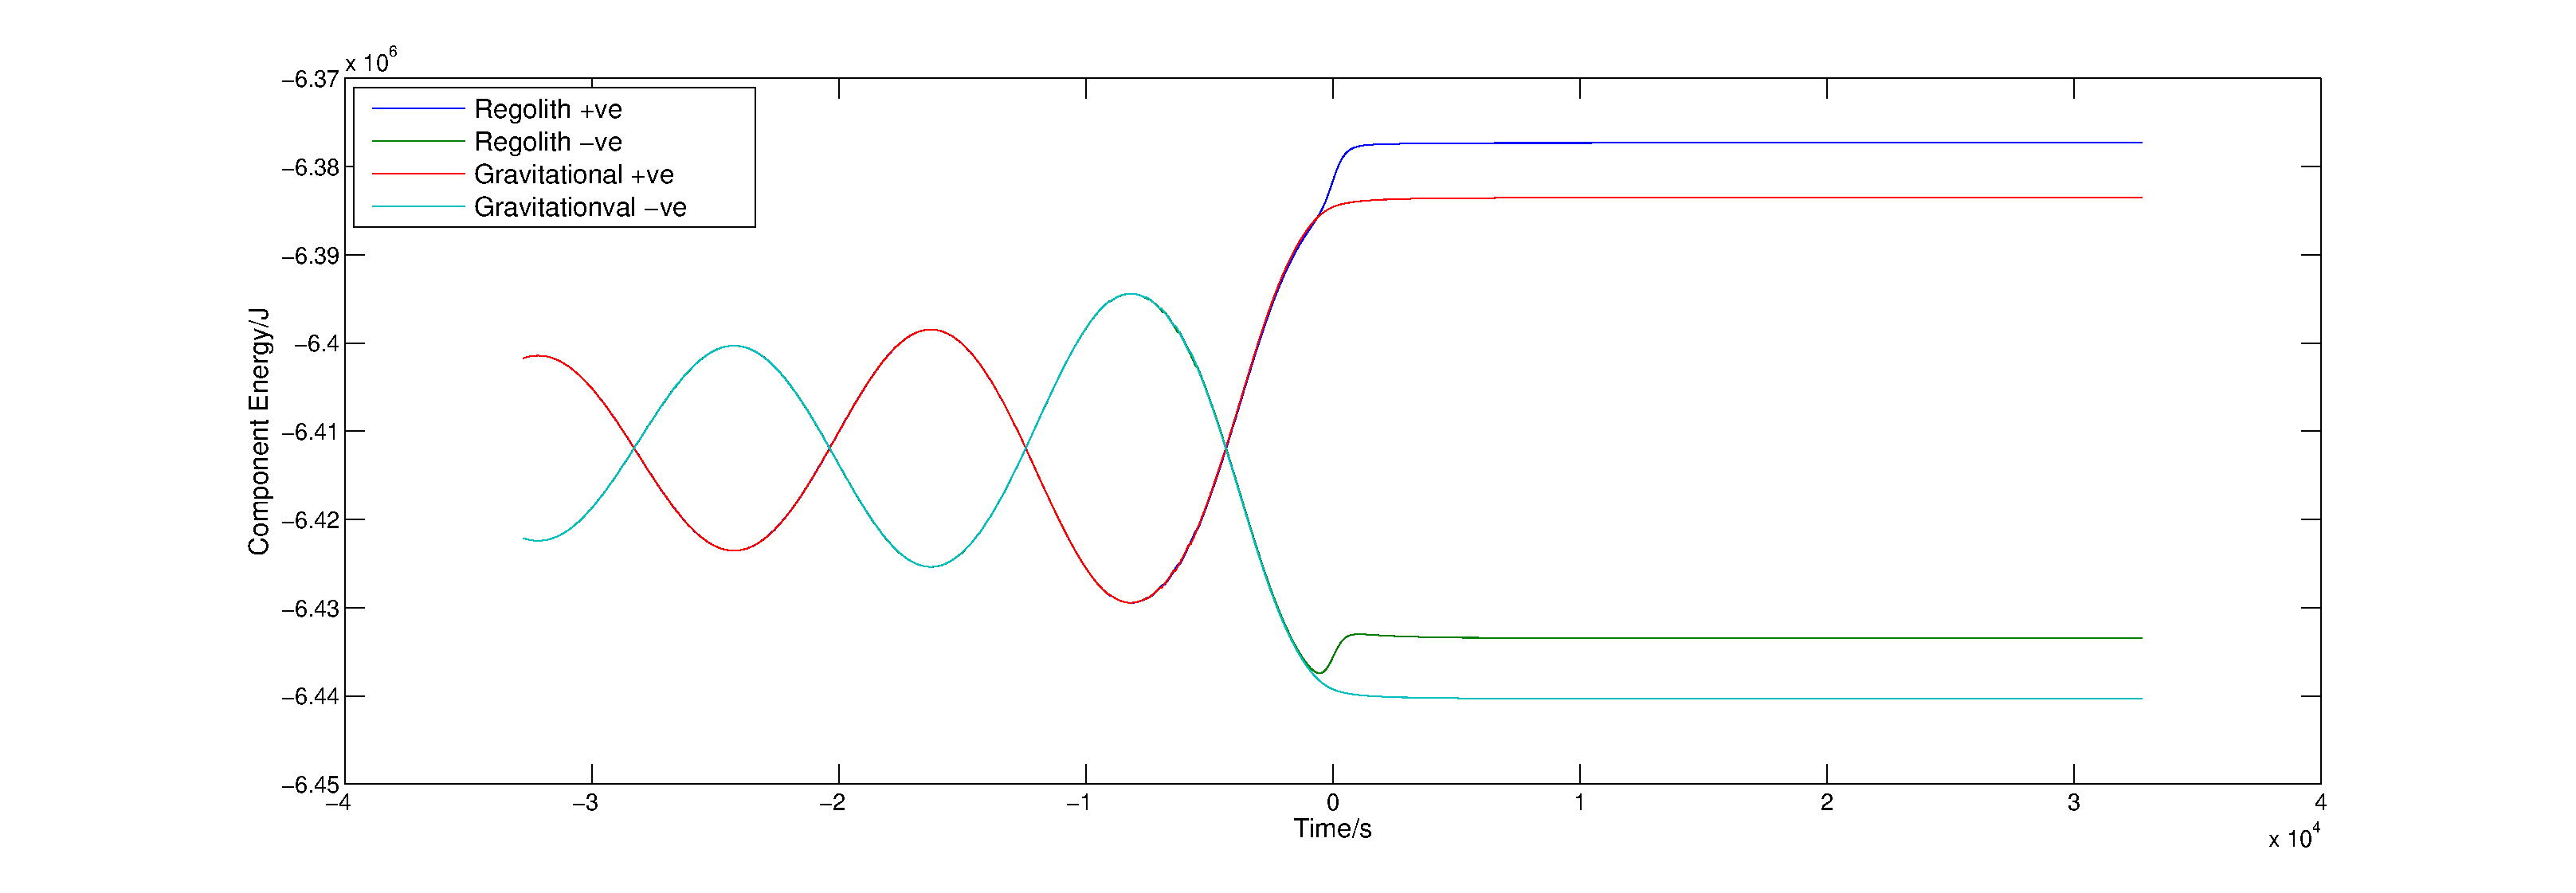
\includegraphics[width=1.2\textwidth]{regolith_v_gravitational.eps}} 
\caption{Plots of the Kinetic energy for two small particles; both bound by a fine regolith bridge and with our force-based approximation for the bridge.} 
\label{fig:dustyspin}
\end{figure}
  
As with the previous encounter simulations, a closest approach distance of 130km is used, and the binary asteroid considered has a total diameter of 4 metres. Figure~\ref{fig:reg} \textbf{\emph{Figure 7 and 8 are the same. I am not sure which one is missing (but i think its 7), but please replace the wrong one}}shows the total energy results from the simulation, compared to those from a simulation of the same binary components and close approach distance but without the regolith bridge. The curves match closely before the fragmentation event; however when fragmentation occurs both binary components gain additional energy from the collapse of the binding regolith bridge. It can be seen that the amount of energy gained from the collapse is about $30\%$ of the difference in total energy between the two components.
 
\begin{figure}[H]
\centering
\centerline{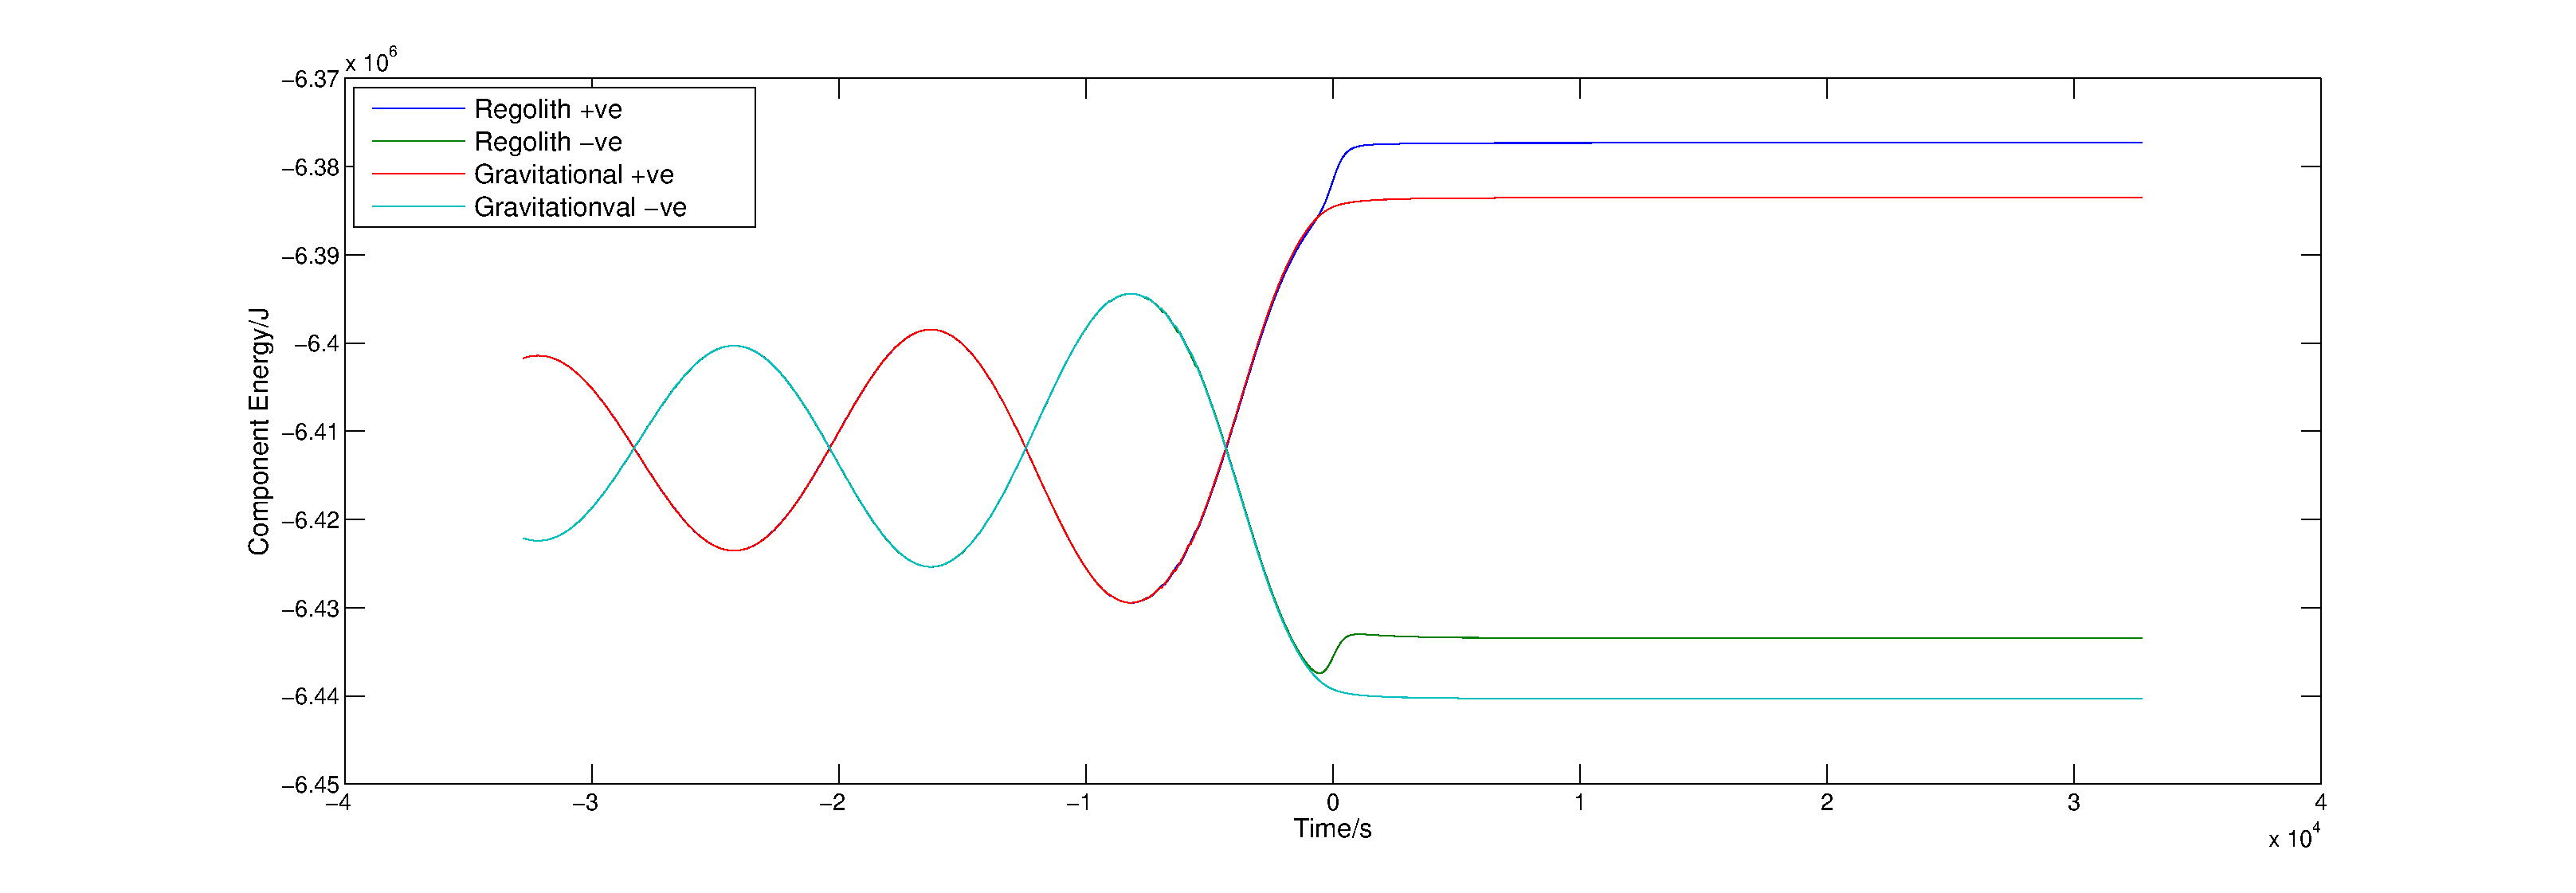
\includegraphics[width=1.2\textwidth]{regolith_v_gravitational.eps}} 
\caption{Plots of the Total energy of both components of the binary from numerical simulations; both for the purely graviational and the regolith-bound cases.} 
\label{fig:reg}
\end{figure}

\subsection{Deflection attempt}

Lastly, we present here a few simulations of attempted deflections for a binary asteroid on a collision course with Earth. Theses simulations are not highly realistic for two main reasons. Firstly, the soft-body collision model does not allow for any permanent deformation, fragmentation or similar phenomena; due to the high velocities required for an impactor-based deflection some degree of deformation would be expected in reality. The second limitation is that of computational time required for simulating the orbit; to minimize this, the deflection is carried out rather close to the Earth (roughly 24 hours before impact). Any real deflection mission would hopefully have significantly more time and as such would require a less aggressive deflection. Still, these simulations indicate certain effects and phenomena which may be present in a more realistic deflection scenario. 

Figure~\ref{fig:bouncey} shows the orbital paths for several cases: an undeflected asteroid, a deflected single-body and both components of a deflected binary. It can be seen that the post-deflection paths of the two components of the binary are greatly different to that of a single body of equal mass. This is likely due to a "Newton's Cradle" type effect in the collisions; as such the component which is struck by the impactor passes all of the additional momentum from the impact to the second, leaving it's momentum largely unchanged by the impact. This effect is most prevalent when the two components are of roughly equivalent mass.
\begin{figure}[H]
\centering
\centerline{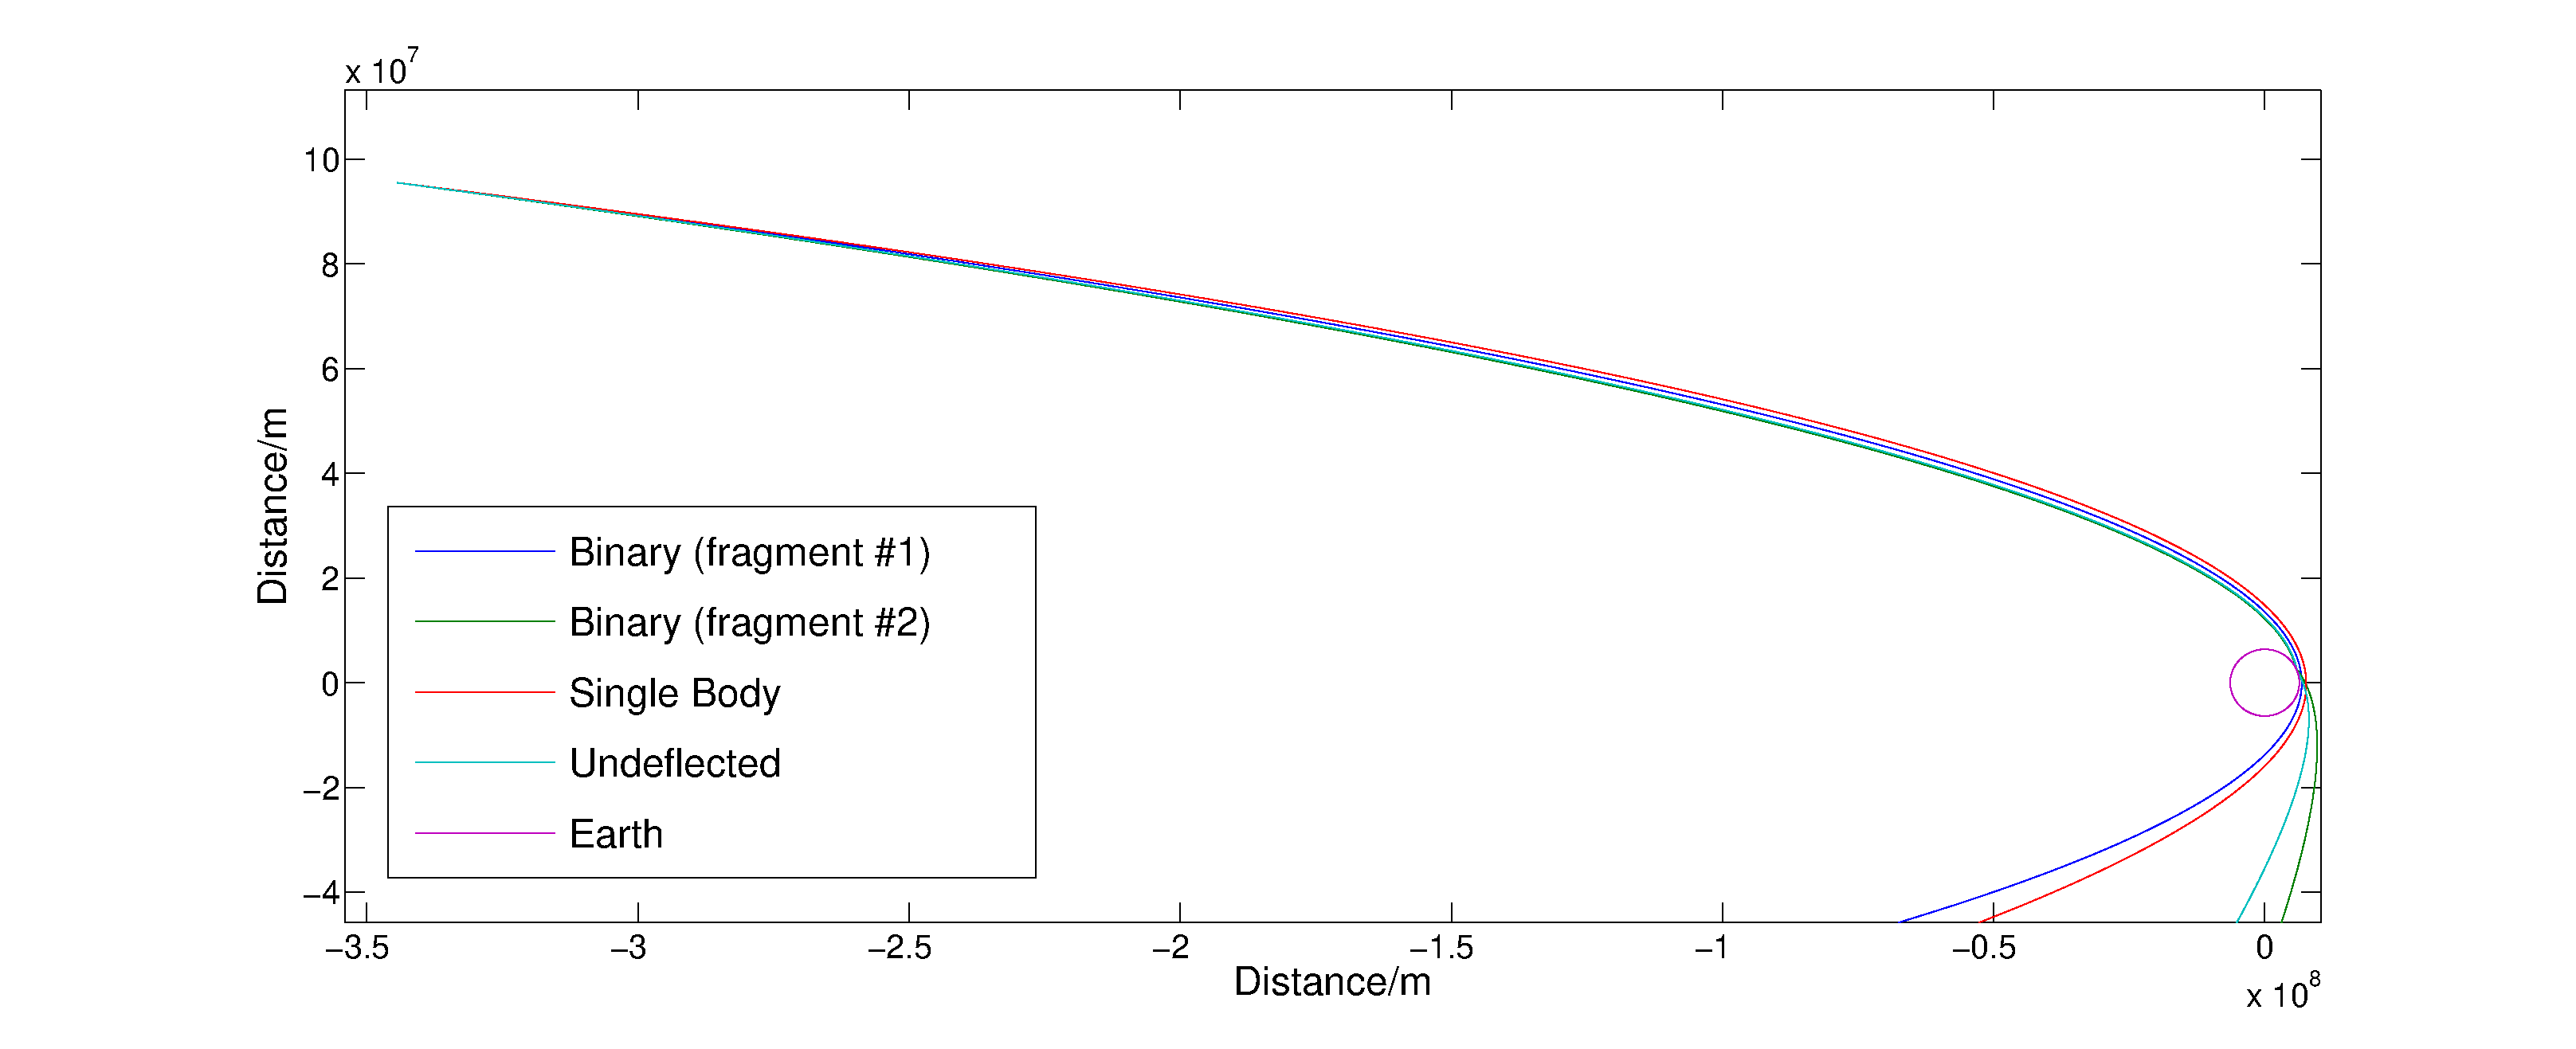
\includegraphics[width=1.2\textwidth]{deflection_1.eps}}
\centerline{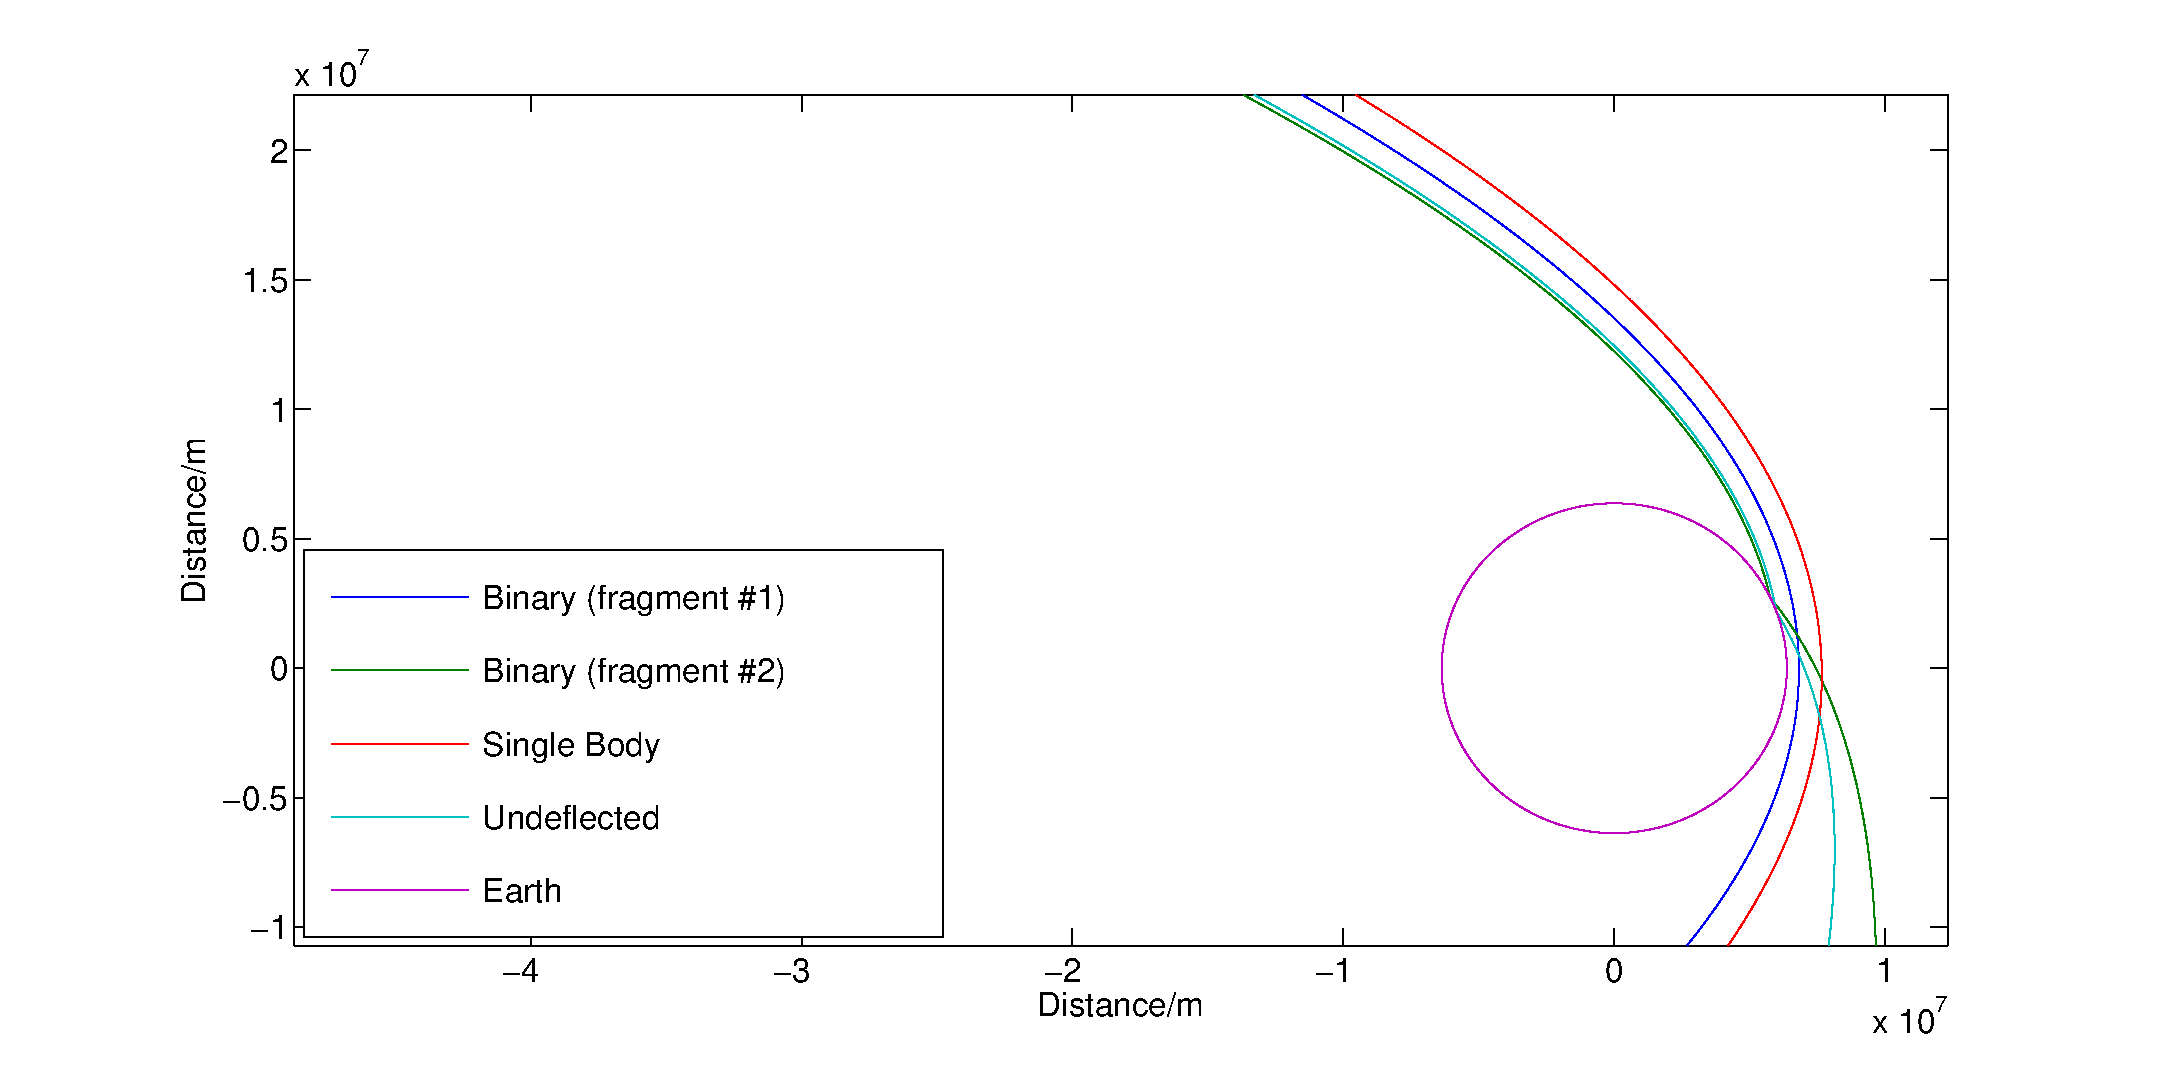
\includegraphics[width=1.2\textwidth]{deflection_0.eps}} 
\caption{Orbital paths of binary and single body asteroids pre and post deflection (fulll orbit and close-up of close encounter/impact.} 
\label{fig:bouncey}
\end{figure} 

We also simulate the effect of an impact on a full regolith-bound binary; both with the same impact speed as the previous case and with a lower speed, more reasonable impact. It can be seen that in both cases, a large amount of the regolith is discharged, and in the former case the bridge fails completely and the pair fragments. \textbf{\emph{is this to be seen in Figure 9? Figure 9 is very confusing, i think it is mislabeled in the legend. the undeflected cyan seems to impact, but why is the green line impacting. the blue and green do not seem like a binary. It seems like they are fragmenting and the deflection is performed before the trajectory that is plotted. The figure needs to show when the fragmentation or deflection occurred.}}

\section{Conclusion}
We present a methodology to model contact binary asteroids bound by regolith during an encounter with a large body such as Earth. Using an analytical approach we have attempted to identify which parameters should impact upon the energy involved in the fragmentation of such an object and the extent of such sensitivity. We find that there the dynamics of the fragmentation event are highly sensitive to the angle of the binary pair with respect to the orbital path, whilst the sensitivity to the closest approach distance and speed of the orbit are much more smooth and in line with the analytical predictions. Also we find that there is a notable change in the fragmentation energy when a full regolith bridge is considered.

Additionally, we give the results of some basic simulations of a deflection attempt. These suggest that the dynamics of an impact-based deflection differ greatly based on whether the object is a single body or a contact binary. 


\bibliographystyle{AAS_publication}   % Number the references.
\bibliography{references_me}   % Use references.bib to resolve the labels.

\end{document}
